\documentclass[10pt,twocolumn,letterpaper]{article}
\usepackage[review]{cvpr}
\usepackage{times,graphicx,amsmath,amssymb,booktabs,microtype,multirow}
\usepackage[accsupp]{axessibility}
\usepackage[pagebackref,breaklinks,colorlinks,allcolors=blue]{hyperref}
\def\paperID{-----}
\def\confName{CVPR}
\def\confYear{2027}
\newcommand{\R}{\mathbb{R}}
\newcommand{\norm}[1]{\left\lVert#1\right\rVert}
\title{Beyond Reconstruction: Auditing Decision and Temporal\\Fidelity in Graph-to-Spike Conversion}
\author{Anonymous authors}
\leftlinenumbers*
\setlength{\linenumbersep}{0.10cm}
\renewcommand\linenumberfont{\fontsize{7}{8}\selectfont\color[rgb]{.5,.5,1}}

\begin{document}
\maketitle

\begin{abstract}
Reconstruction error is widely used to assess ANN-to-SNN conversion, but does a more accurate reconstruction necessarily preserve the computation of a graph classifier? We investigate this question through a finite-event audit of frozen graph neural networks on visual superpixel graphs. Our audit applies realizable event interventions while keeping the task computation fixed. First, legal one-event modifications that reduce the actual next-message error nevertheless worsen the teacher-class margin in 40.9\% and 31.9\% of message-improving interventions on MNIST and CIFAR-10, respectively. A directional margin analysis explains why a smaller graph-propagated error need not favor the teacher's decision. Second, exchanging source-verified two-tick codewords with identical local decoded tensors and equal local event counts changes downstream predictions and whole-network activity. These exchanges preserve the local endpoint but differ in intermediate prefixes and absolute amplitudes, exposing information omitted by terminal reconstruction. Complementary calibration and residual-centering studies illustrate the implications for conversion design. Together, our findings motivate an evaluation framework that distinguishes reconstruction fidelity, decision fidelity, intermediate-prefix behavior, and whole-network activity.
\end{abstract}

\section{Introduction}
A smaller reconstruction error can produce a worse classification decision. Consider a converted graph classifier operating on an MNIST superpixel graph. Changing a single event by one legal amplitude level reduces the error of the next graph message, yet moves the teacher-class margin from $+1.97$ to $-3.75$ and changes the prediction from digit 5 to digit 4. An even stronger constraint can fail: two event sequences that reconstruct exactly the same local activation at the final tick and emit the same number of events can still produce different downstream predictions. As illustrated in Fig.~\ref{fig:concept}, these examples expose a basic question in graph-to-spike conversion: what does local reconstruction actually preserve?

Converting pretrained artificial neural networks into spiking or event-driven networks offers a way to reuse learned representations without retraining the original weights~\cite{li2021,wu2024ftbc,huang2025}. For visual graph classifiers, conversion must preserve not only node activations but also the computation carried through graph propagation and readout~\cite{dwivedi2023}. Existing calibration, bias-correction, and differential-coding methods have substantially improved conversion fidelity~\cite{bojkovic2024,hao2023residual,li2024erroraware}. Nevertheless, the finite-prefix regime remains challenging. In our superpixel graph classifiers, four active ticks already recover nearly the original ANN accuracy, whereas a single tick leaves a substantial performance gap. This regime provides a controlled setting in which to examine the quantities preserved by conversion.

Two distinctions motivate our analysis. First, a reconstruction norm summarizes the size of an approximation error but discards its signed direction relative to the classifier's decision boundaries. Even when the error is measured after the actual graph operator, a smaller norm need not improve the relevant class margin. Second, a terminal decoded activation summarizes an event sequence without specifying the intermediate signals encountered by its downstream consumers. Stateful event units can respond differently to these intermediate signals before local equality is restored. Reconstruction fidelity is therefore related to, but does not determine, either decision fidelity or downstream computational equivalence.

We introduce a finite-event audit that tests these distinctions through realizable interventions in a frozen converted graph model. The graph, pretrained weights, and underlying event recurrence remain fixed. For decision fidelity, we modify an existing event by one legal amplitude level and replay the downstream computation, measuring the resulting graph-message error, teacher-class margin, and prediction. For temporal fidelity, we exchange source-verified codewords with identical local decoded endpoints and event counts, allowing their downstream states to evolve normally. The two tests examine complementary failure modes of reconstruction-based evaluation: an improved local metric and an exactly matched local endpoint.

Our experiments reveal that neither form of local fidelity is sufficient to determine downstream behavior. Across the tested intervention distributions, 40.9\% of message-improving changes on MNIST and 31.9\% on CIFAR-10 worsen the teacher-class margin at the first tick. The effect appears under both deterministic-coordinate and largest-residual selection, with different rates across intervention rules. In the temporal test, exchanging all eligible amplitude-reducing codewords changes six of 128 MNIST predictions and 16 of 128 CIFAR-10 predictions, while increasing whole-network activity by 3.41\% and 4.99\%, respectively. These results distinguish local reconstruction, intermediate computation, and global model behavior within the frozen conversion setting.

These observations motivate a broader evaluation principle: conversion quality should be assessed at the level at which the converted model is required to operate. We therefore examine teacher agreement and task accuracy separately, measure decisions at the required prefixes, and distinguish local event counts from whole-network activity and measured execution cost. Complementary studies of calibration objectives and residual centering show how this perspective informs the evaluation of conversion strategies.
\begin{figure*}[t]
\centering
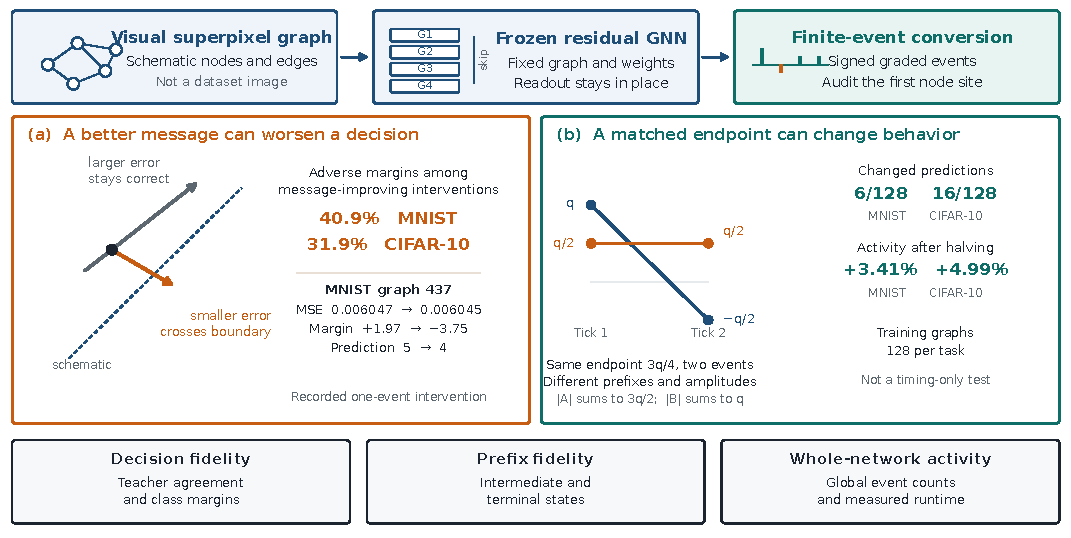
\includegraphics[width=\textwidth]{figures/concept.pdf}
\caption{A finite-event audit beyond local reconstruction. We examine a frozen graph classifier converted to a finite-event computation. (a) A legal one-event modification can reduce the actual next-message error while worsening the teacher-class margin or changing the prediction. The highlighted example is a recorded MNIST intervention; displayed margins are rounded, and Sec.~\ref{sec:decision-results} reports the full values. The boundary drawing is schematic. (b) Source-verified codewords can share an identical local decoded endpoint and event count while presenting different intermediate prefixes and absolute amplitudes. Exchanging all eligible codewords changes predictions and whole-network activity on 128 training graphs per task. The two tests separate decision fidelity, prefix fidelity, and global activity from local reconstruction.}
\label{fig:concept}
\end{figure*}

Our contributions are threefold:
\begin{itemize}
\item We formulate a finite-event audit for frozen graph-to-spike conversion, combining graph-propagated approximation errors, directional class margins, and realizable event interventions.
\item We establish controlled decision and temporal counterexamples on visual graph classifiers: reducing next-message error can worsen the teacher-class margin, while exact local terminal decoding and matched event counts can coexist with different downstream predictions.
\item We show how these distinctions affect conversion evaluation, including prefix-wise fidelity and whole-network activity, and examine their implications through complementary calibration and residual-centering studies.
\end{itemize}

\section{Related Work}
\paragraph{Conversion and finite-prefix fidelity.}
ANN-to-SNN conversion has developed a range of strategies for reducing approximation error at short time horizons. Layerwise calibration matches pretrained ANN responses~\cite{li2021}; distribution-based threshold and potential initialization, forward temporal bias correction, and error-aware parameter calibration address related mismatches~\cite{bojkovic2024,wu2024ftbc,li2024erroraware}. Residual membrane readout preserves information discarded by integer spike counts~\cite{hao2023residual}. Differential coding with graded events supplies the event unit adapted in our graph converter~\cite{huang2025}. One-Spike SNN is a separate single-spike phase-coding converter that also demonstrates GCN conversion~\cite{hwang2025onespike}; our one-event edits are diagnostic interventions inside a differential-coding adapter, not an implementation of that converter. These methods address complementary sources of conversion error. Our study asks a different question: which properties of the downstream computation are determined by local reconstruction under finite-event constraints?

\paragraph{Reconstruction and decision preservation.}
Prediction-aware quantization has shown that local feature reconstruction and global prediction quality need not favor the same approximation parameters. PD-Quant selects quantization parameters from prediction differences rather than layerwise reconstruction~\cite{liu2023pdquant}. Degree-Quant and A$^2$Q account for graph aggregation when designing quantized graph networks~\cite{degreequant2021,a2q2023}. Building on these observations, we examine legal event-level modifications rather than optimizing a new quantization objective. This tests whether reducing the actual graph-message error preserves the decision of a frozen converted classifier. Feature-only and relabeled-operator controls later separate the role of the true adjacency from the fitting budget.

\paragraph{Temporal alignment and stateful computation.}
Temporal misalignment and feature--output alignment highlight the intermediate signals consumed by spiking networks~\cite{bojkovic2025,li2026cka}. Inference-scale complexity analysis further separates local activity from the cost of a complete converted network~\cite{bu2025complexity}. Our temporal test imposes a complementary constraint: the exchanged codewords must be source-realizable and must preserve both the local terminal decoded tensor and the local event count. We then evaluate whether these local equivalences extend to downstream predictions and whole-network activity. The test leaves absolute amplitude and the first-prefix profile free, so it examines endpoint equivalence rather than a pure timing intervention.

\section{Finite-Event Fidelity Audit}
We audit conversion fidelity by intervening on the finite-event representation of a frozen graph classifier. Rather than introducing new trainable weights or a new event encoder, the audit asks which downstream properties survive a realizable local modification. We consider two complementary interventions: changing one legal event to test decision sensitivity, and exchanging exactly endpoint-equivalent codewords to test downstream temporal behavior. Both interventions are evaluated by executing the original graph computation.

\subsection{Frozen graph computation and event semantics}
Our primary testbed is a frozen residual GCN for visual superpixel classification. The graph operator and pretrained weights are preserved throughout the audit, so changes in downstream behavior can be attributed to the finite-event modification. The teacher has four residual graph-convolution layers of width 146. For fixed normalized adjacency $A$, its evaluation-mode layer is
\begin{equation}
 H_{\ell+1}=H_\ell+\operatorname{ReLU}(AH_\ell W_\ell^\top+b_\ell),
 \label{eq:block}
\end{equation}
with batch normalization folded into $W_\ell,b_\ell$. Node features and positions are embedded together. Mean pooling feeds a 146--73--36--10 MLP with two hidden ReLUs. The conversion exposes four node activation sites and two readout sites. Its graph operator weights each original directed edge $u\!\to\!v$ by $[\max(d_{\rm out}(u),1)\max(d_{\rm in}(v),1)]^{-1/2}$, without adding self-loops. The residual path supplies the identity connection.

The event alphabet contains signed graded amplitudes $\{0,\pm\theta,\ldots,\pm\theta/128\}$, with per-channel threshold $\theta>0$, rather than binary spikes. An event count therefore measures the number of nonzero scalar emissions, not a hardware operation or an energy cost. We call the total number of nonzero scalar events \emph{whole-network activity}. Let $c_t$ be the current at active tick $t$, and let $(v,C,a,b)$ denote membrane, cumulative output, integrated input, and integrated output states. The source differential unit first computes
\begin{equation}
 m=v+c_t+a-b,\qquad \widetilde C=C+b.
\end{equation}
It emits the largest eligible magnitude $s_t$. A positive level $q=\theta 2^{-k}$ requires $m\geq 0.75q$; a negative level requires $m\leq -0.75q$ and $\widetilde C\geq q$. The updates are
\begin{equation}
\begin{split}
 v&\leftarrow m-s_t,\quad C\leftarrow\widetilde C+s_t,\\
 a&\leftarrow a+c_t/t,\quad b\leftarrow b+s_t/t.
\end{split}\label{eq:state}
\end{equation}
The decoder is $D_T(s)=\sum_{t=1}^T s_t/t$. Raw inputs and affine biases enter once, at the first active tick. We use $T$ for the number of active ticks, not measured latency. Residual and readout arithmetic remains continuous where the adapter specifies it.
\subsection{Decision audit}
\label{sec:decision}
A graph-message reconstruction metric measures how closely a converted activation reproduces the next propagated representation. The decision depends on how that approximation changes the relative logits of competing classes. We separate the magnitude of a propagated perturbation from its direction in decision space.

For an activation perturbation $E$ relative to the pre-intervention converted activation at a fixed site, the immediate next-message perturbation is
\begin{equation}
 \Delta M=AEW^\top.\label{eq:message}
\end{equation}
Thus $\norm{\Delta M}_F^2$ accounts for the actual propagation operator, but compresses a signed, graph-dependent perturbation into one scalar. For a linear graph readout $R$, the induced logit change in that linear region is $\Delta z=RAEW^\top$. This identity is elementary. Its role here is to show which information a norm omits.

Let $y$ be the teacher class and let $z$ denote the pre-intervention converted logits. The margin against competitor $k\neq y$ is $m_k=z_y-z_k$. After a perturbation that changes the logits by $\Delta z$, the converted prediction agrees with $y$ when
\begin{equation}
 m_k+\Delta z_y-\Delta z_k>0\quad\text{for all }k\neq y,
 \label{eq:margin}
\end{equation}
apart from ties. In a locally linear region, write $\Delta z=J\operatorname{vec}(E)$, where $J$ includes the graph operator and readout. The decision depends on the signed projections $(J_y-J_k)\operatorname{vec}(E)$, not on the reconstruction norm alone. A sufficient condition is
\begin{equation}
 \norm{\operatorname{vec}(E)}_2<
 \min_{k\neq y}\frac{m_k}{\norm{J_y-J_k}_2},\label{eq:sufficient}
\end{equation}
when the corresponding row is nonzero; a zero row imposes no restriction. A smaller norm tightens this worst-case bound. It does not order two perturbations that point in different directions. Later hard-event boundaries can also change $J$, so Eq.~\eqref{eq:margin} is the exact decision condition we use, and every reported intervention is measured by replaying the hard forward pass.

For each intervention, the scalar teacher-class margin is the converted logit of the teacher's predicted class minus the largest competing converted logit. The strongest competitor may change after the intervention. Margin deterioration is not the same as a prediction change, and disagreement with the teacher is not the same as an error relative to the ground-truth label. A converted prediction can disagree with an incorrect teacher and become correct. We therefore report teacher agreement and ground-truth accuracy separately.

The same margin view connects to early rate-coding analysis. Under a nonsaturating constant-drive integrator, rate error scales with $\theta/T$, and retaining the membrane residual removes the final count quantization. Combining a valid hidden-error envelope with Eq.~\eqref{eq:sufficient} yields a sufficient time budget that depends on propagation and margin. It does not imply one time budget or a row-stochastic bound for every graph: symmetric degree normalization is not generally row stochastic. The supplement records the assumptions and the historical node-classification results.

\subsection{Temporal audit}
The decision audit shows that improving a local error metric need not preserve the classifier's decision. We now impose a stronger constraint, exact equality of the local terminal decoded representation. In a stateful event network, that equality still leaves the intermediate inputs and internal trajectories unspecified.

Equation~\eqref{eq:state} stores more than a decoded terminal activation. Replacing a first-tick event by $s_1+\delta$ also changes $v\leftarrow v-\delta$, $C\leftarrow C+\delta$, and $b\leftarrow b+\delta$. A later event therefore depends on both the incoming history and the internal state. Matching $D_T(s)$ at one site cannot by itself match the intermediate currents received by its consumers.

A scalar counterexample uses the frozen source recurrence, $\theta=1$, zero initial state, and $T=2$. The input histories $(c_1,c_2)=(0.01,1.58)$ and $(1,-0.4)$ have the same integrated input $c_1+c_2/2=0.8$. Both emit two nonzero events, yet the decoded outputs are $0.5078125$ and $0.75$. A threshold at $0.6$ separates them. Thus matching integrated input and event count does not determine even the decoded output of a stateful nonlinear consumer. This example is not the codeword exchange used on the graph models: it preserves integrated input, whereas the graph test preserves the decoded output.

To examine state dependence inside a converted graph classifier, we use source-verified first-site codewords
\begin{equation}
 (q,-q/2)\quad\longleftrightarrow\quad(q/2,q/2).
 \label{eq:words}
\end{equation}
Both decode to $3q/4$ at the second tick and contain exactly two nonzero events (Fig.~\ref{fig:temporal-mechanism}). Their first-prefix values differ, and their unweighted absolute amplitudes sum to $3q/2$ and $q$. We exchange a codeword only when every level belongs to the original alphabet and source replay, under the known zero second-tick input, produces the required second event. Both directions are checked. The subsequent forward pass executes normally and does not reset downstream states. Equality at every consumed tick, together with identical initial state, would preserve a deterministic downstream trajectory. Equality only at the terminal tick does not. The controlled conclusion is therefore narrower than a claim about timing alone.

\begin{figure}[t]
\centering
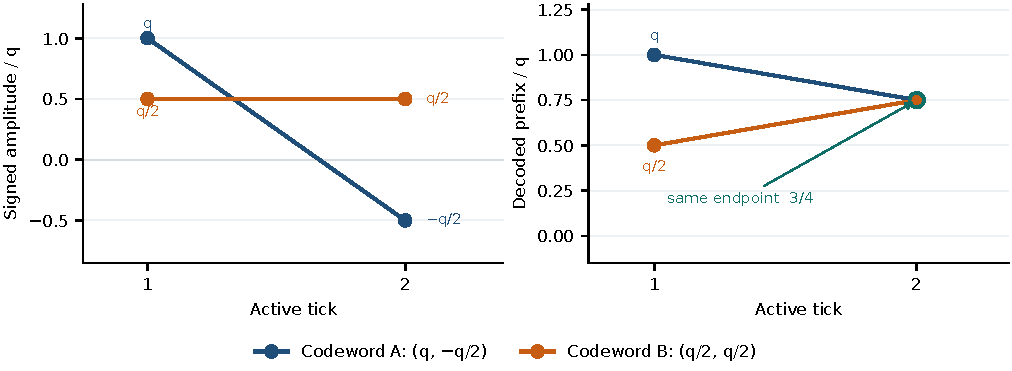
\includegraphics[width=\linewidth]{figures/temporal_mechanism.pdf}
\caption{Exact local endpoint equivalence under different event prefixes. The two source-verified codewords contain two nonzero events and decode to the same terminal value, $3q/4$, while producing different first-prefix values and absolute amplitudes. Eligible exchanges preserve local decoding and event count; the remaining network evolves without a state reset.}
\label{fig:temporal-mechanism}
\end{figure}

\subsection{Realizable interventions and evaluation protocol}
Given a frozen graph classifier, the audit has four steps: identify an eligible event site, construct a realizable local intervention, replay the downstream computation with its original state updates, and measure message error, decision margins, prefix-wise predictions, and global activity.

We report three evidence levels, detailed in the supplement. Full historical test predictions from three teacher seeds characterize conversion fidelity, and full-validation position interventions localize conditional sensitivity. Single-teacher hard interventions use 512 fixed validation graphs per task, giving 2{,}048 first-tick attempts. Exact codeword tests use 128 training graphs per task. The centered-residual profile uses all 45{,}000 CIFAR-10 training graphs of one GatedGCN teacher. Official validation and test splits were exposed during development. Their results are descriptive evidence, not a new blind test.

For position analysis, an ideal causal ReLU replaces one selected converted activation while the graph, weights, and incoming converted computation stay fixed. It is a continuous diagnostic, not a deployable finite-event repair. Restoring all six sites reproduces the ANN. Group effects are nonadditive because each intervention changes the computation that follows.

For the hard intervention, we move one existing nonzero first-site event up or down by one legal amplitude level, update the affected states, and replay the network. The coordinate is either deterministic or the largest eligible local residual. Upward and downward moves can have different eligible sets. The teacher is used only afterward, to score margin and agreement. Confidence intervals resample graphs and keep each graph's repeated interventions together.

Calibration controls share teacher weights, histogram thresholds, 512 training graphs, 693 initial-potential offsets, and 64 Adam updates. The offsets are $\theta\rho$ with $\rho\in[-0.5,0.5]$. Local fitting averages normalized site MSE, graph-output fitting targets teacher logits, and the mixed objective uses both. A second family fits an immediate-message objective and compares the actual $A$ with the identity and a within-graph conjugation $P^{-1}AP$. The task graph itself is unchanged.
\section{Auditing Finite-Event Graph Conversion}
\subsection{Where short-prefix conversion loses accuracy}
Before applying the audit, we locate the regime in which conversion error is most consequential. The visual graph classifiers recover nearly their original ANN accuracy at four and eight active ticks, whereas one tick leaves a substantial gap (Table~\ref{tab:main}). We therefore focus on the first few prefixes, where a local approximation must still pass through the remaining graph computation. Table~\ref{tab:main} reports aggregate accuracy. Close aggregate accuracy does not mean that every converted prediction matches the ANN.

\begin{table}[t]
\caption{Historical full-test accuracy (\%), mean $\pm$ sample standard deviation over three teacher seeds on the same 10{,}000 graphs. These tests were previously exposed. GatedGCN is a separate hybrid adapter with continuous gates.}
\label{tab:main}
\centering\small
\setlength{\tabcolsep}{4pt}
\begin{tabular}{lrrr}\toprule
Task / teacher & ANN & $T{=}4$ & $T{=}8$\\\midrule
MNIST / GCN & $91.02\pm.27$ & $91.05\pm.26$ & $91.02\pm.26$\\
CIFAR-10 / GCN & $54.94\pm.07$ & $54.92\pm.08$ & $54.97\pm.05$\\
CIFAR-10 / Gated & $68.77\pm.41$ & $68.75\pm.33$ & $68.76\pm.39$\\\bottomrule
\end{tabular}
\end{table}

At one tick, fixed-GCN conversion falls to $71.44\pm2.80\%$ on MNIST and $46.80\pm1.22\%$ on CIFAR-10. On the full 5{,}000-graph validation split of each teacher, restoring the first node activation closes 54.08\% and 23.54\% of the teacher-disagreement gap. Restoring all four node sites closes 80.4\% and 45.2\%; restoring both readout sites closes 8.8\% and 14.9\% (Fig.~\ref{fig:positions}). The first node activation is the largest single-site recovery in these models, which is why the later event interventions target it. The recovery uses a continuous response and is not itself a finite-event correction. Group effects are nonadditive.

\begin{figure}[t]
\centering
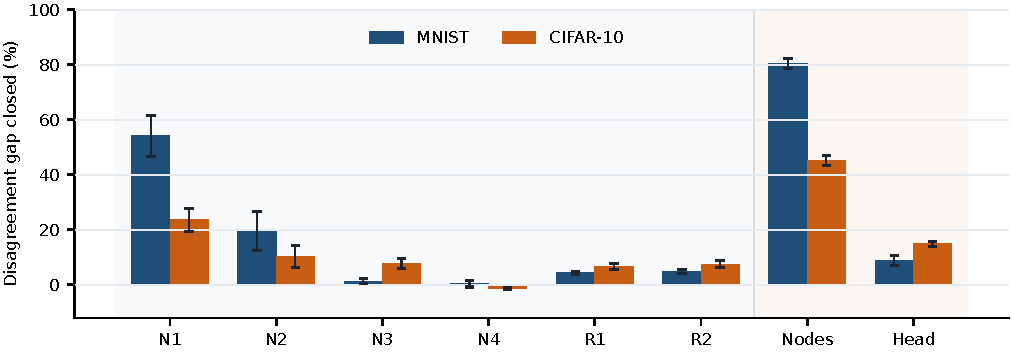
\includegraphics[width=\linewidth]{figures/position_recovery.pdf}
\caption{The first node activation is the most sensitive single site at one tick. Continuous position recovery measures the fraction of the teacher-disagreement gap closed by restoring individual sites or groups. Bars average three teachers on the full validation splits; error bars are sample standard deviations. The shaded region on the right restores four node sites or both readout sites. Group effects are nonadditive.}
\label{fig:positions}
\end{figure}

Classical node classification supplies a compatible but separate observation. Audited historical two-layer integrate-and-fire experiments approach their own ANN teachers at longer horizons when analytic bias compensation and membrane readout are used. Cora, for example, reaches 80.16\% at $T{=}8$ against an 80.46\% teacher. The decoder and time scale differ from Table~\ref{tab:main}. The supplement keeps that separation.

\subsection{Can a better graph message worsen the decision?}
\label{sec:decision-results}
If the first node site is influential, a natural correction is to reduce the approximation error of the message it sends onward. We test whether that improvement also favors the teacher's decision by changing one existing event by a single legal amplitude level.

Among the 2{,}048 attempted interventions per task, 811 MNIST and 928 CIFAR-10 interventions reduce the actual first-tick message MSE. Of those improvements, 332 and 296 worsen the teacher-class margin, or 40.94\% and 31.90\%. The graph-cluster bootstrap 95\% intervals are $[37.28,44.57]\%$ and $[28.66,35.31]\%$. The same first-tick modifications worsen the second-prefix margin in 48.71\% and 44.07\% of these message-improving cases (Table~\ref{tab:hard}). The second-prefix rates retain the first-tick message condition; they are not rates among second-prefix reconstruction improvements, and they are not model error rates.

\begin{table}[t]
\caption{Lowering first-tick message MSE can worsen the teacher-class margin. Both prefixes use the first-tick improvement condition. Each task has 512 graphs and 2{,}048 attempts. Intervals are 95\% graph-cluster bootstrap intervals.}
\label{tab:hard}
\centering\small
\setlength{\tabcolsep}{2.2pt}
\begin{tabular}{llrl}\toprule
Task & Readout & Adverse / improved & Rate [interval] (\%)\\\midrule
MNIST & $T{=}1$ & 332 / 811 & 40.94 [37.28, 44.57]\\
 & $T{=}2$ & 395 / 811 & 48.71 [45.02, 52.42]\\
CIFAR-10 & $T{=}1$ & 296 / 928 & 31.90 [28.66, 35.31]\\
 & $T{=}2$ & 409 / 928 & 44.07 [40.54, 47.60]\\\bottomrule
\end{tabular}
\end{table}

The mismatch is not confined to predictions that are nearly tied. On MNIST validation graph 437, the teacher and the ground truth both identify digit 5, and the teacher's top-two margin is 5.20378. A deterministic downward event modification reduces the next-message MSE from 0.00604723 to 0.00604511, while the converted teacher-class margin changes from 1.97242 to $-3.74764$. The converted prediction changes from digit 5 to digit 4. A locally favorable modification can move the executed hard-event computation across a decision boundary.

The phenomenon appears under all four tested rule--direction combinations, but its frequency depends on the eligible interventions (Fig.~\ref{fig:hard-strat}). At the first tick, deterministic-coordinate selection has adverse rates of 30.6\% downward and 36.2\% upward on MNIST, and 20.4\% and 24.7\% on CIFAR-10. Largest-residual selection is higher in every direction: 49.0\% and 48.5\% on MNIST, and 42.6\% and 38.5\% on CIFAR-10. At the graph level, 50.2\% of MNIST graphs and 42.2\% of CIFAR-10 graphs contain at least one adverse message-improving intervention, while 7.8\% and 12.7\% contain at least one prediction change under these fixed rules. The intervention distribution is part of the result.

\begin{figure}[t]
\centering
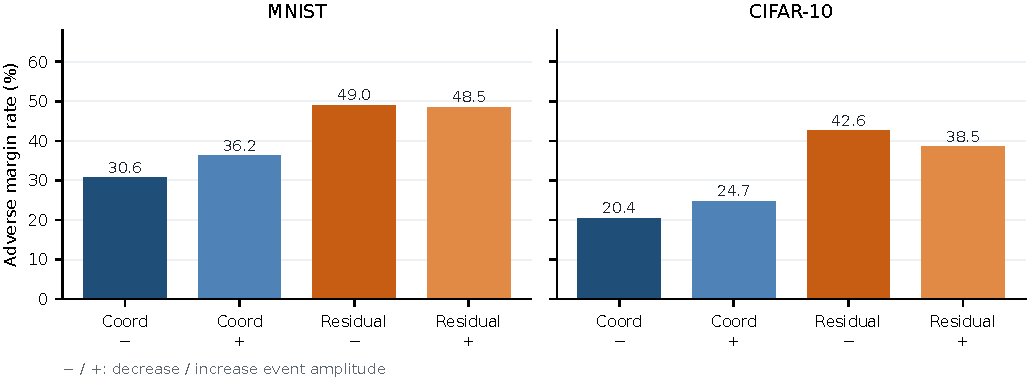
\includegraphics[width=\linewidth]{figures/hard_intervention_stratified.pdf}
\caption{Adverse decision directions depend on the intervention rule. Rates use first-tick message-improving interventions, separately for deterministic-coordinate and largest-residual selection in each amplitude direction. One teacher and 512 previously exposed validation graphs are used per task.}
\label{fig:hard-strat}
\end{figure}

Aggregate gains can coexist with harmful individual modifications. Relative to local allocation, actual-message allocation reduces normalized message MSE from 0.001378 to 0.001280 on MNIST and from 0.002018 to 0.001717 on CIFAR-10. On CIFAR-10, 491 of 512 graphs improve this metric, yet 27 of those change from correct to incorrect. The corresponding MNIST counts are 440 and 17. Gains on other graphs can offset these losses in mean accuracy. The audit therefore reveals prediction-level effects that aggregate reconstruction and accuracy can hide.
\subsection{Does decision-aware calibration remove the mismatch?}
The interventions suggest that calibration should see the downstream prediction. We ask whether replacing or combining the local reconstruction objective with a graph-output objective gives a consistent advantage under matched calibration resources.

Under that matched budget, output and mixed objectives produce small, setting-dependent changes relative to local fitting (Table~\ref{tab:calibration}). Output-minus-local differences on the full historical tests are $+0.20$ and $+0.18$ percentage points at MNIST $T{=}1$ and $T{=}2$, and $-0.18$ and $+0.19$ on CIFAR-10. Full-validation differences are $-0.10$, $-0.13$, $-0.27$, and $+0.43$ in the same order. No tested objective dominates across both tasks and prefixes. Teacher agreement and ground-truth accuracy can also move in opposite directions: fitting logits at the first two ticks raises one-tick accuracy by 1.17 points on each task relative to strong local fitting, while CIFAR-10 teacher agreement falls by 2.15 points.

\begin{table}[t]
\caption{Matched local, output, and mixed objectives. Accuracy (\%) is mean $\pm$ sample standard deviation over three teachers on historical full tests. Every objective uses 693 offsets, 512 training graphs, and 64 updates, and each horizon is calibrated separately.}
\label{tab:calibration}
\centering\small
\setlength{\tabcolsep}{3.5pt}
\begin{tabular}{llrrr}\toprule
Task & $T$ & Local & Output & Mixed\\\midrule
MNIST & 1 & $78.50\pm2.10$ & $78.70\pm2.19$ & $78.95\pm2.08$\\
 & 2 & $90.08\pm.26$ & $90.26\pm.35$ & $90.19\pm.44$\\
CIFAR-10 & 1 & $49.92\pm.14$ & $49.75\pm.68$ & $49.72\pm.32$\\
 & 2 & $54.18\pm.14$ & $54.37\pm.26$ & $54.42\pm.25$\\\bottomrule
\end{tabular}
\end{table}

A top-two ranking objective makes the same point for competing classes. It decreases its hard training loss, yet the fraction of predictions outside the teacher's top two rises from 4.69\% to 22.95\% on MNIST and from 9.47\% to 27.34\% on CIFAR-10. Improving a loss defined around two classes leaves the other competitors in Eq.~\eqref{eq:margin} unconstrained.

The operator controls separate a related distinction. Actual-message allocation is close to conjugated allocation on MNIST (79.49\% versus 79.30\%) and equal to feature-only allocation on CIFAR-10 (49.22\%). The actual graph operator defines the immediate message perturbation, but using it as an allocation objective does not by itself produce a consistent aggregate-accuracy advantage over these alternatives. Reconstructed degree and neighborhood variables add little in-sample explanatory power after the teacher margin, with incremental $R^2$ values of 0.004--0.035. A source threshold-iteration control, using its original moment estimates, 100 updates, and fallback rules, yields one-tick accuracies of 71.48\% and 45.31\% and four-tick accuracies of 91.21\% and 54.88\%. High-prefix fidelity and a severe first-prefix gap therefore coexist under more than one calibration rule.

\subsection{Does exact local decoding preserve the network?}
Improving a reconstruction metric does not guarantee a better decision. We now ask whether exact local reconstruction is a stronger guarantee. Source-verified codeword exchanges hold the first-site two-tick decoded tensor and the local nonzero event count fixed, while every subsequent event state evolves normally.

The eligible pools contain 84{,}905 first-site coordinates on MNIST and 132{,}899 on CIFAR-10 for the amplitude-reducing exchange, and 55{,}510 and 63{,}500 for the amplitude-increasing exchange. Source replay records a maximum absolute decoded-tensor error of zero, so the local terminal values match exactly. The first-prefix profile and the unweighted absolute amplitude are not controlled.

Despite that local equality, the amplitude-reducing exchange changes 6 of 128 MNIST predictions and 16 of 128 CIFAR-10 predictions (Fig.~\ref{fig:temporal-decisions}). The reverse exchange changes 2 and 10 predictions. On MNIST, the reducing exchange gains and loses three teacher agreements. On CIFAR-10 it loses seven and gains six: ground-truth accuracy rises from 66.41\% to 67.97\%, while teacher agreement falls from 85.16\% to 84.38\%. Mean accuracy does not reveal these paired decision changes.

\begin{figure}[t]
\centering
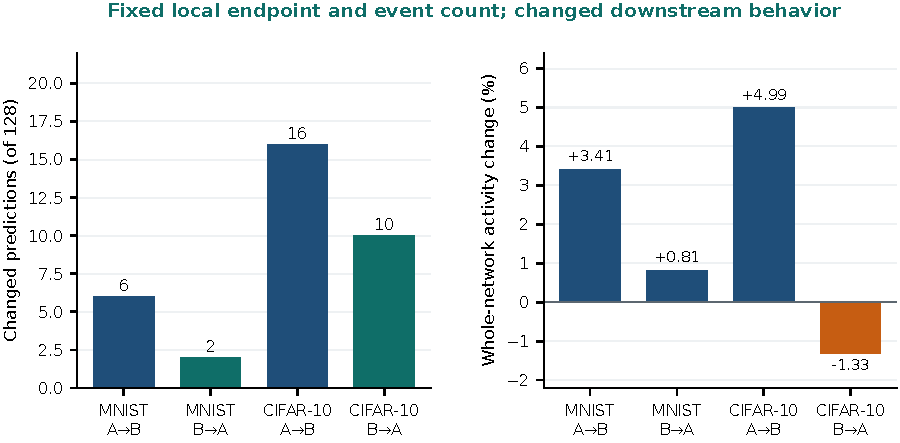
\includegraphics[width=\linewidth]{figures/temporal_decision_effects.pdf}
\caption{Exact local codeword equivalence changes downstream decisions and activity. Each exchange preserves the local two-tick decoded tensor and local event count. Both directions are evaluated on 128 training graphs per task. Activity is the change in nonzero scalar events over the whole network.}
\label{fig:temporal-decisions}
\end{figure}

The same exchanges fail to determine global activity. Replacing every eligible codeword in the amplitude-reducing direction raises the total number of nonzero events from 4{,}351{,}056 to 4{,}499{,}463 on MNIST and from 6{,}876{,}233 to 7{,}219{,}258 on CIFAR-10, increases of 3.41\% and 4.99\%. The amplitude-increasing exchange raises MNIST activity by 0.81\% and lowers CIFAR-10 activity by 1.33\%. Neither the local event count nor a reduction in unweighted local amplitude determines whole-network activity.

A terminal decoder retains a weighted sum of emitted events. It does not specify the intermediate currents received by downstream units. Those units update their internal states at every tick, so different source prefixes can lead to different later computations before first-site equality is restored. Because our codewords also differ in absolute amplitude, the experiment does not isolate timing from amplitude. Its controlled statement is that terminal equality together with a fixed local event count does not establish downstream equivalence.

\subsection{Residual centering as a constructive application}
The preceding results motivate a further question: which part of a representation needs to be encoded? Residual graph architectures give a concrete case. Write $h_\ell=h_0+q_\ell$, where $q_\ell$ accumulates nonnegative residual-branch increments. For a projection,
\begin{equation}
 Wh_\ell+b=(Wh_0+b)+Wq_\ell.\label{eq:center}
\end{equation}
The initial representation can act as a static carrier, while subsequent residual increments are the coded inputs. Equation~\eqref{eq:center} is an affine identity. Caching the carrier and sharing one residual stream within a layer are implementation choices, not new algebra. Continuous gates, products, normalization, and readout still belong to the full computation.

Under shared channel thresholds, centered coding lowers logit MSE and prospective coded-projection additions at every tested prefix, $T\in\{1,2,4\}$, for threshold scales 1 and 8 (Fig.~\ref{fig:centered}). At scale 1 and $T{=}1$, teacher agreement rises by 2.04 points, while projected additions fall from $9.099\times10^{11}$ to $6.650\times10^{11}$ across the 45{,}000-graph training split. Agreement improves in five of the six comparisons and decreases by 0.0044 points at scale 1, $T{=}4$. The choice of representation origin changes both reconstruction and one component of arithmetic work. The projected additions exclude the static carrier and the rest of inference, so they are not a measured energy or latency saving.

\begin{figure}[t]
\centering
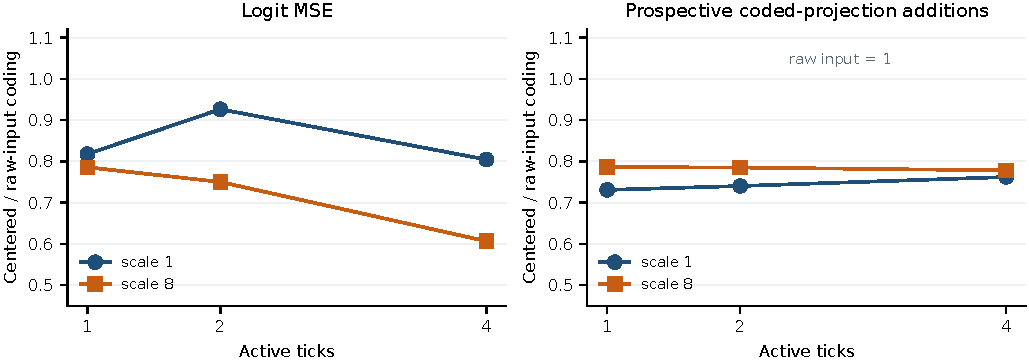
\includegraphics[width=\linewidth]{figures/centered_tradeoff.pdf}
\caption{Residual centering reduces logit error and prospective coded-projection work under shared thresholds. Ratios below one favor centered coding. The dashed line is the raw-input reference. Results use one CIFAR-10 GatedGCN teacher and the full training split. Projection additions count the specified coded operations.}
\label{fig:centered}
\end{figure}

A separate three-teacher campaign evaluates centered conversion on all 5{,}000 exposed CIFAR-10 validation graphs. At $T{=}4$ and $T{=}8$, centered mean accuracy is 70.53\% and 70.56\%, within 0.07 and 0.05 points of the strongest recorded controls. Its matched dense implementation takes 6.245 and 12.049 ms per graph, against 6.213 and 3.132 ms for those controls. The campaign leaves a complete efficiency advantage unresolved. These controls use their own calibration and head conventions and are kept separate from Fig.~\ref{fig:centered} and Table~\ref{tab:main}.

\subsection{From local event counts to execution cost}
The activity changes in the codeword audit raise a practical measurement question. In the current implementation, graph projections are evaluated densely at every active tick, so a zero event does not skip a kernel. On an RTX 3060, synchronized cached-batch timings average 0.152 and 0.157 ms per graph for the MNIST and CIFAR-10 ANNs, against 0.366 and 0.493 ms at $T{=}1$ and 1.238 and 1.762 ms at $T{=}4$ for the diagnostic converter. Each number averages three seed-level medians, using 32-graph batches and 30 interleaved repeats. The timings include decoded-site accumulation, exclude transfer and loading, and are not optimized deployment bounds. No chip energy is measured.

Event allocation has the same separation. In its matched timing experiment, actual-message allocation costs 0.834 and 0.991 ms per graph, against 0.668 and 0.806 ms for local allocation. These measurements distinguish the number of active ticks, scalar event activity, prospective coded-projection operations, and measured execution time. Each captures a different aspect of conversion cost.

\section{Discussion}
The finite-event audit exposes two complementary limitations of reconstruction-based conversion evaluation. The first concerns decision direction: a graph-message error norm measures the magnitude of a perturbation but does not specify its effect on competing class logits. The second concerns state history: an identical local decoded endpoint does not specify the intermediate signals consumed by downstream event units. These distinctions arise from different mechanisms, yet both show why reconstruction alone cannot certify the behavior of a finite-event computation.

The findings have direct implications for conversion design. Position recovery can identify influential activation sites, while realizable event interventions test whether a local correction favors the required decision. Endpoint-equivalent codewords provide a way to examine downstream state dependence without changing the local terminal reconstruction or the local event count. The calibration and residual-centering studies show how the same perspective can assess a proposed conversion strategy across fidelity and cost measures.

The scope of the evidence is frozen superpixel graph classifiers and the studied signed graded-event adapters. The main hard-intervention experiments use one teacher per task and fixed validation or training graphs, while the three-teacher studies characterize conversion fidelity and conditional position sensitivity. The codeword exchanges preserve terminal decoding and event count, but not absolute amplitude or the first-prefix profile. Extending the tests to other converters, teacher populations, and feature-dependent graph operators remains open. Within the studied setting, the audit makes decision, prefix, and activity visible where message fidelity and local terminal equality do not.

\section{Conclusion}
Graph-to-spike conversion requires more than accurate local reconstruction. Through realizable finite-event interventions, we show that reducing graph-message error can worsen a classifier's decision, and that identical local decoded endpoints with equal event counts can still produce different downstream predictions and activity. Directional class margins and the stateful event recurrence explain why these local measures omit decision-relevant and temporal information. The audit therefore motivates evaluating conversion through prefix-wise decision fidelity and whole-network activity alongside reconstruction accuracy.

\section*{LLM Usage Statement}
OpenAI Codex was used for research-asset inspection, analysis and figure code, evidence checks, mathematical discussion, drafting, and compilation. OpenAI ChatGPT assisted with the final narrative, language editing, and the conceptual layout of the overview figure. The submitted figures were redrawn programmatically from recorded tables and explicit mathematical examples; no generated image is included, and no experimental value came from a language or image model. Earlier reviews used Kimi K3.1 Pro, DeepSeek V4.1 Flash, WorkBuddy, Claude, and Grok. Historical records do not identify every model version from those stages. Human authors remain responsible for all claims, citations, code, disclosures, and any submission.

{\small
\bibliographystyle{ieeenat_fullname}
\bibliography{references}}
\end{document}